\section{Reducing The Branching Factor}
The branching factor associated with each tile on the perimeter of an empty room (in an 8-connected 
grid map) is dependent on the dimensions of the room.
Consider an empty room of width $w$ and height $h$ where $w > h$.
After adding all non-dominated macro edges to the room, each tile is incident with at least $h$ macro edges and up to $2h-1$ 
depending on its positon on the perimeter.
Further, each tile is adjacent with 2 other tiles from the perimeter of the same room and up to 3 tiles from an adjacent room.
Thus the total branching factor for each tile is at least $h + 2$ and can be as high
as $2h + 4$.
Generally speaking, a large branching factor is undesirable for two reasons:
(i) invididual node expansion operations take longer and (ii) additional neighbours usually 
add more branches to the search tree and make it more difficult to reach the goal.
\par
In this section we discuss two novel optimality preserving methods for reducing branching factor. 
The first is an offline perimeter reduction method while the second is an online optimisation which speeds up 
node expansion when searching along the perimeter of an empty room.
We will discuss both methods in the context of 8-connected grid maps.
Analogous algorithms, suitable to 4-connected grid maps, are easily derived.
\par \noindent \newline
\textbf{Perimeter Reduction:}
We observe that in many cases there are tiles on the perimeter of an empty room which have no neighbours from any 
adjacent room. 
These tiles represent intermediate locations between entry and exit points that lead into and out of each empty room.
To speed up search we propose pruning from the perimeter of each room all such nodes.
To preserve optimality, we will connect the neighbours of each pruned node directly to each other.
The weight of each new edge is therefore equal to the octile distance between the two neighbours.
Figure \ref{fig-reduction} shows an example.
This is a very simple optimisation but as we will see, it can have a dramatic effect on the average performance of
A* on certain types of maps.

\begin{figure}[t]
       \begin{center}
                       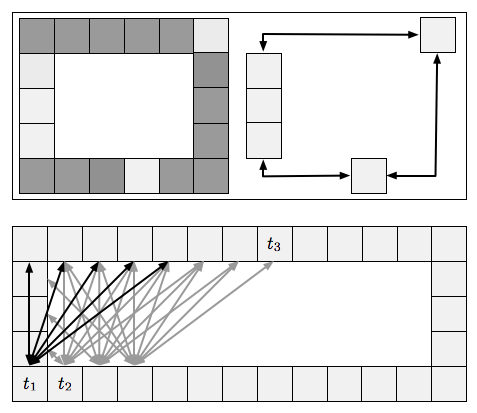
\includegraphics[scale=0.5, trim = 10mm 10mm 10mm 0mm]{diagrams/branching.png}
       \end{center}
	\vspace{-3pt}
       \caption{(Top) An empty room. Dark grey tiles have no neighbours from any adjacent room. 
We prune these nodes and connect their neighbours directly (not all macro edges shown).
		(Bottom) A path enters an empty room at tile $t1$ and exits at tile $t2$. Notice that once
$t1$ is expanded every path to $t2$ is dominated by a path that starts at $t1$ and mentions one of its macro edges.
}
       \label{fig-branching}
\end{figure}

\par \noindent \newline
\textbf{Faster Node Expansion:} 
We noted earlier that the number of neighbours associated with a tile on the perimeter of an empty room grows linearly
with the dimensions of the room. 
However, as Figure \ref{fig-branching} (Bottom) shows, many of these neighbours are often on a dominated or symmetric
path during the search instance at hand.
We therefore propose the following symmetry elimination technique to speed up node expansion:
\begin{enumerate}
\item{Divide the set of neighbours associated with each tile on the perimeter of an empty room into two distinct sets:
\emph{primary neighbours} and \emph{secondary neighbours}.
Secondary neighbours are those which are located on the opposite side of the room to the current tile. 
Primary neighbours are all the rest.}
\item{When expanding a node, determine which room the parent of the current node belongs to.}
\item{If the parent and the current node belong to different rooms process all primary and secondary neighbours.
However, if the parent and the current node belong to the same room, process only primary neighbours.}
\end{enumerate}

\begin{lemma}
The ''Fast Node Expansion'' algorithm preserves optimality during search.
\end{lemma}
\begin{proof}
There are three cases to consider:
\begin{enumerate}
\item{$m$ and $n$ are on the same side of the room}
\item{$m$ and $n$ are on orthogonal sides of the room}
\item{$m$ and $n$ are on opposite sides of the room}
\end{enumerate}
In all cases we begin by expanding $m$ and process all its primary and secondary neighbours.
Subsequent nodes from the same room, which are descendants of $m$ in the search tree, 
only have their primary neighbours evaluated during expansion.
In the first and second case the optimal path from $m$ to $n$ involves no tiles from the opposite side of the room;
the decision to ignore all secondary neighbours has no effect on the optimality of the solution.
In the third case we argue as follows:
if $m$ and $n$ are connected by a macro edge, an optimal path is found when we expand $m$.
When this is not the case we can simply follow one of the macro edges at $m$ to a node $n'$ which on the same side
of the room as $n$ and from there travel along the perimeter to $n$.
The only alternative way to reach $n$ is to travel along the perimeter from $m$ to some node $m'$ and follow
a macro edge from $m'$ directly to $n$. 
It is simple to show however that the length of these two paths are equal.
Thus, the decision to ignore all secondary neighbours for all possible choices of $m'$ has no effect on the optimality
of the solution.
\end{proof}


